\begin{frame}{example graphs}
\begin{itemize}
\item lots of things can be represented as graphs
\end{itemize}
\end{frame}

\begin{frame}{maps}
\begin{tikzpicture}
\node[inner sep=0mm] (the map) {
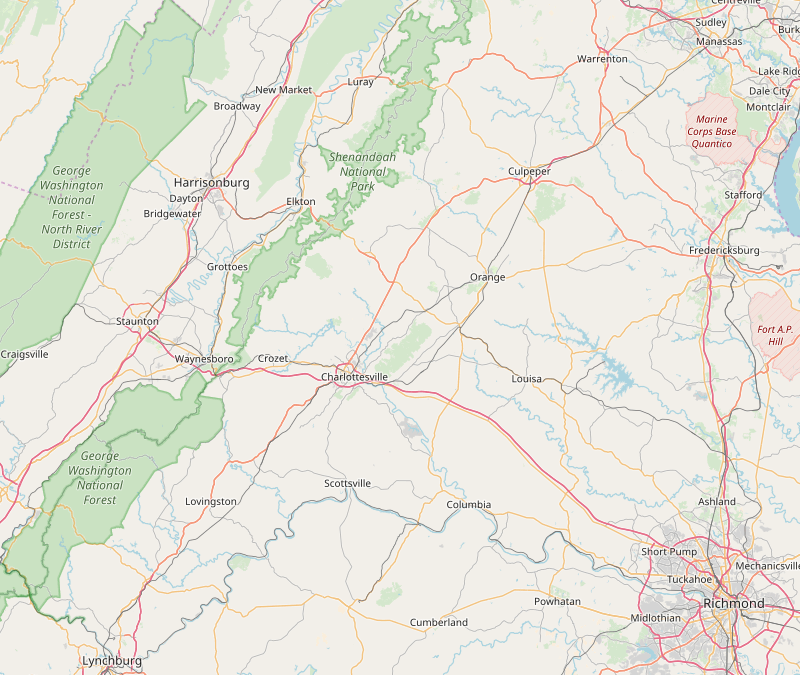
\includegraphics[height=\textheight]{map-example}
};
\node[align=left,right=0cm of the map] {
    nodes: intersections? \\
    edges: roads?
};
\end{tikzpicture}
\imagecredit{image: open street map}
\end{frame}

\begin{frame}{airline routes}
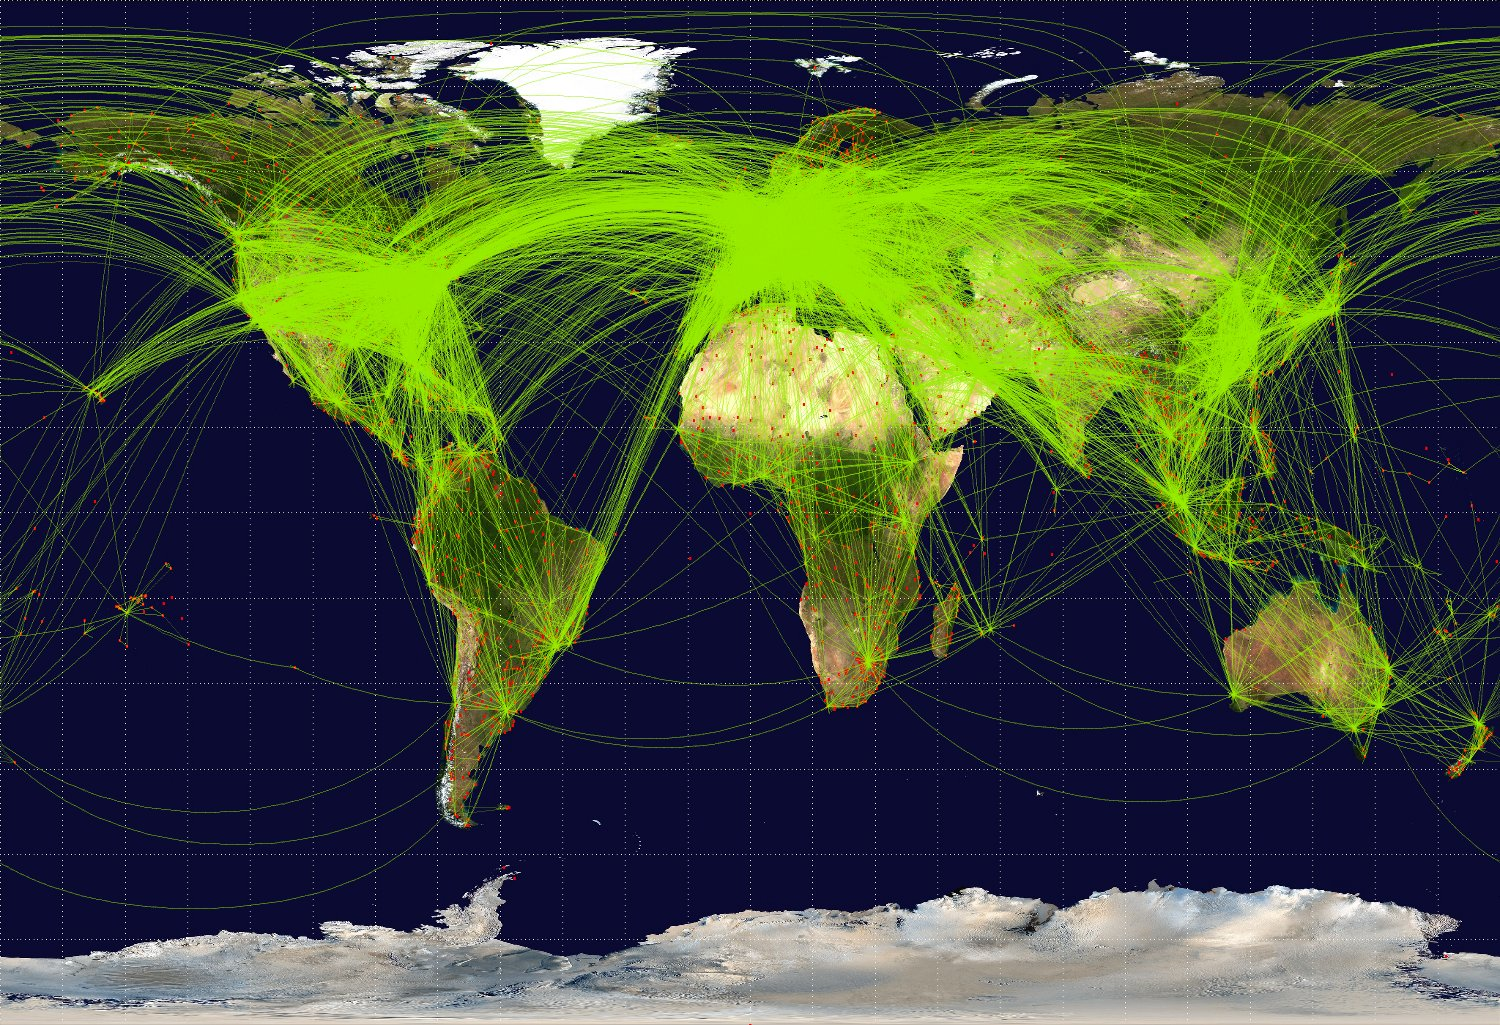
\includegraphics[height=0.9\textheight]{airline-routes-from-openflights}
\imagecredit{image: openflights}
\end{frame}

\begin{frame}{flowcharts}
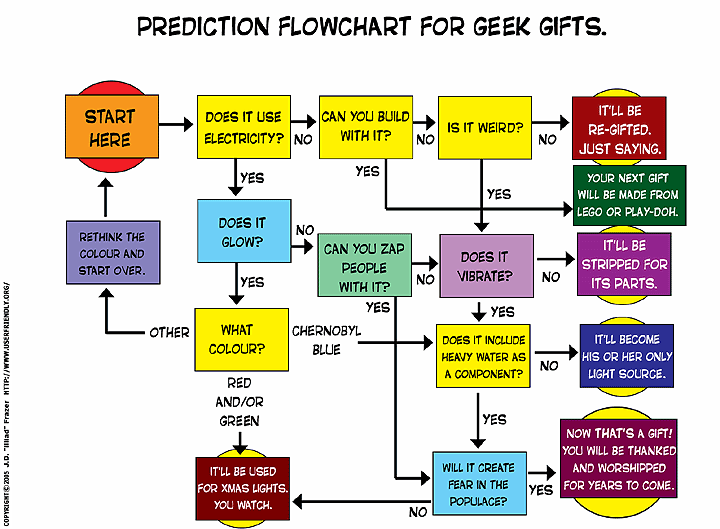
\includegraphics[height=0.9\textheight]{geek-gift-flowchart}
\end{frame}

\begin{frame}{pre-requisite tree}
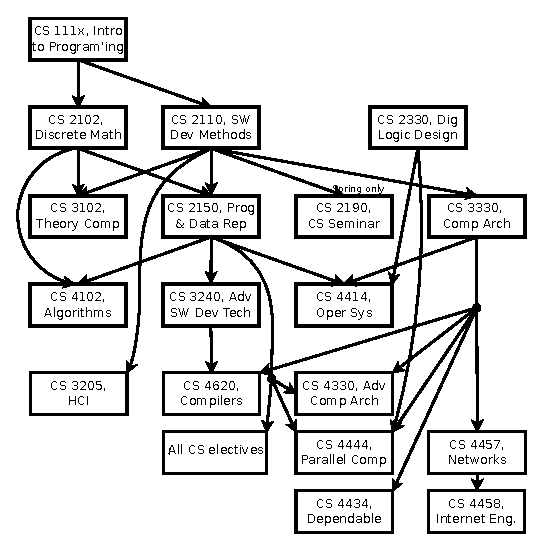
\includegraphics[height=0.9\textheight]{bs-cs-chart}
\end{frame}
